\documentclass[10pt,fleqn]{beamer}

\hypersetup{pdfpagemode=FullScreen}
\beamertemplatenavigationsymbolsempty
\usetheme{mcgill}
\DeclareGraphicsExtensions{.jpg,.eps,.png,.pdf,.mps,.gif}

\usepackage[latin1]{inputenc}
\usepackage[T1]{fontenc}
\usepackage[english]{babel}
\usepackage{pgf,pgfarrows,pgfnodes,pgfautomata,pgfheaps}
\usepackage{amsmath}
\usepackage{amsfonts}
\usepackage{graphicx}
\usepackage{epsfig}
\usepackage{subfigure}
\usepackage{color}
\usepackage{lmodern}
\usepackage[3D]{movie15}
\usepackage{ragged2e} %文本两端对齐 \justifying
\usepackage{booktabs} %19-24行 为表格模板所需要的包
\usepackage{cellspace}
\usepackage{pgf}
\usepackage{tikz}
\setlength\cellspacetoplimit{3pt}
\setlength\cellspacebottomlimit{3pt}
\usepackage{makecell}
\setcellgapes{3pt}

%%%%%%%%%%%%%%%%%%%%%%%%%%%%%%%%%%%%%%%%%%%%%%%%%%%%%%%%%%%%%%%%%%%%%%%%%%%%%%%%%%%%%%%
% color definitions %%%%%%%%%%%%%%%%%%%%%%%%%%%%%%%%%%%%%%%%%%%%%%%%%%%%%%%%%%%%%%%%%%%
%%%%%%%%%%%%%%%%%%%%%%%%%%%%%%%%%%%%%%%%%%%%%%%%%%%%%%%%%%%%%%%%%%%%%%%%%%%%%%%%%%%%%%%
\definecolor{gris1}{RGB}{220,220,220}
\definecolor{gris2}{RGB}{180,180,180}
\definecolor{couleurtitreslide}{RGB}{220,220,220}
\definecolor{couleurrouge}{RGB}{210,0,0}
\definecolor{couleurtexteblock}{RGB}{145,5,5}
\definecolor{couleurfond}{RGB}{255,255,255}

%%%%%%%%%%%%%%%%%%%%%%%%%%%%%%%%%%%%%%%%%%%%%%%%%%%%%%%%%%%%%%%%%%%%%%%%%%%%%%%%%%%%%%%
% title page definition %%%%%%%%%%%%%%%%%%%%%%%%%%%%%%%%%%%%%%%%%%%%%%%%%%%%%%%%%%%%%%%
%%%%%%%%%%%%%%%%%%%%%%%%%%%%%%%%%%%%%%%%%%%%%%%%%%%%%%%%%%%%%%%%%%%%%%%%%%%%%%%%%%%%%%%
\setbeamercovered{dynamic}
\setbeamerfont{author}{family=\rmfamily}

\author[authors: Tianma Shen]{authors: Tianma Shen\\[5pt]\scriptsize{University of Shanghai for Science and Technology}}%首页的名字和底部的名字
\title[Learning Report ]{Learning Report From SEP. TO OCT.}%首页的题目和底部的题目
\institute{%conference name\\
\small{}} % 首页中间一行字(被我隐藏有需要可以添加)
\date[2017.9]{2017.10.13} %首页日期和底部日期
\titlegraphic{
\includegraphics[height=2cm]{logo}}%logo为eps文件,首页logo

% table of contents depth
\setcounter{tocdepth}{1}

\begin{document}
	\usebackgroundtemplate{
\includegraphics[width=160mm]{McGillBackground}}%背景eps
	\frame[plain]{\titlepage}

	\part{Main Part}
	\frame{\frametitle{Outline}\tableofcontents}

	\section{CNN Architecture}%第一标题
	\subsection{FakeTitle1} % subtitles are not used in this layout but still required for the header outline bullets
	\frame{
\frametitle{CNN Architecture 1998-2014}%此页的标题

\begin{figure}
	\begin{center}
		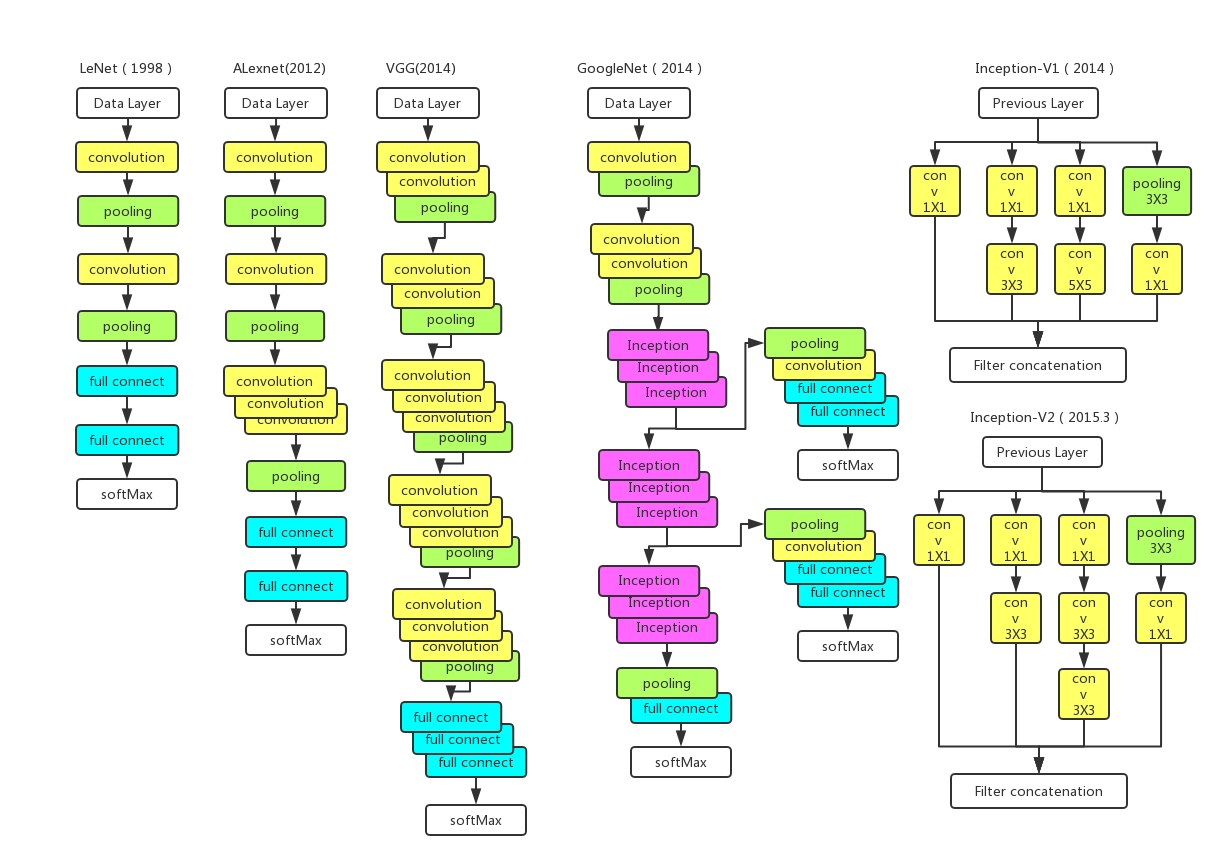
\includegraphics[width=0.9\linewidth]{picture//Architecture1.png}
		% \caption{Knowledge Graph of Machine Learning}
		% \label{Fig:1}
	\end{center}
	% \vspace{-0.1em}
\end{figure}

}%第一标题第一页,名字在对应tex中修改
	\frame{
\frametitle{Inception}%此页的标题

\begin{figure}
	\begin{center}
		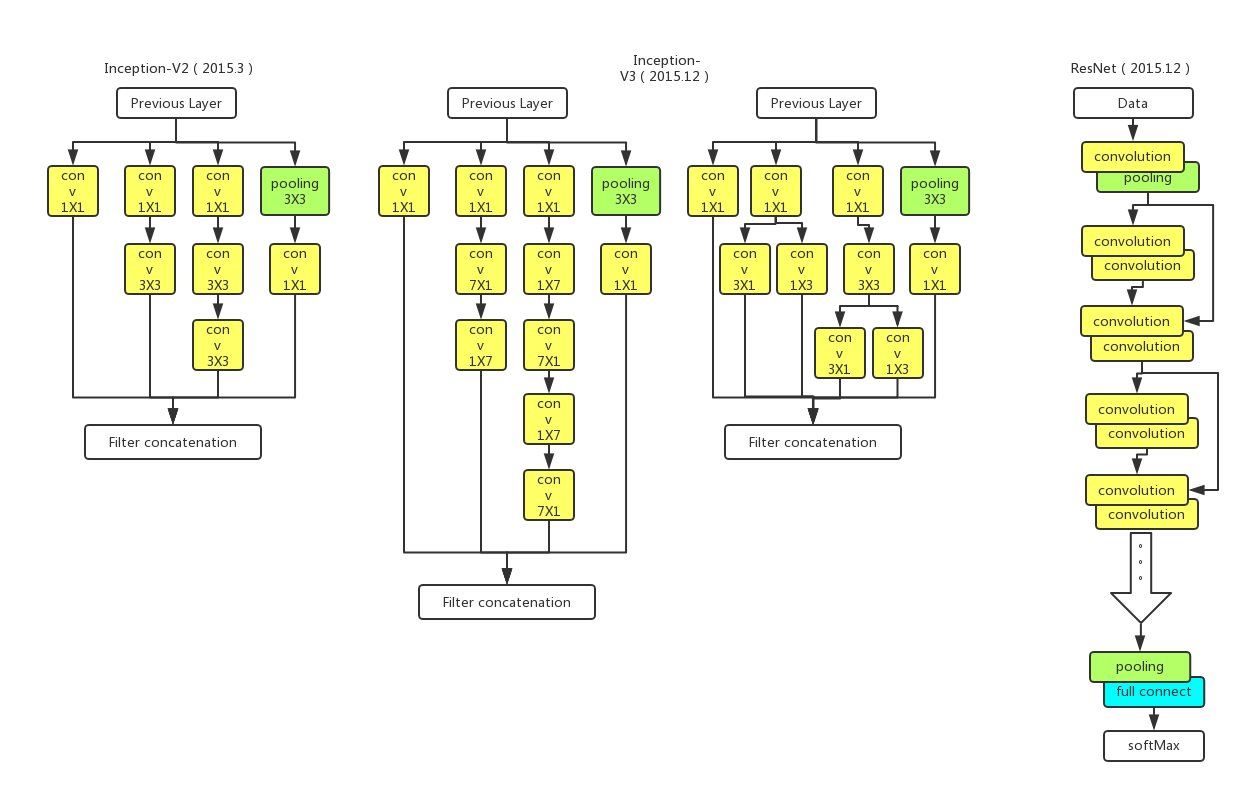
\includegraphics[width=1\linewidth]{picture//Inception.png}
		% \caption{Knowledge Graph of Machine Learning}
		% \label{Fig:1}
	\end{center}
	% \vspace{-0.1em}
\end{figure}

}
	\frame{
\frametitle{ResNet}%此页的标题

\begin{figure}
	\begin{center}
		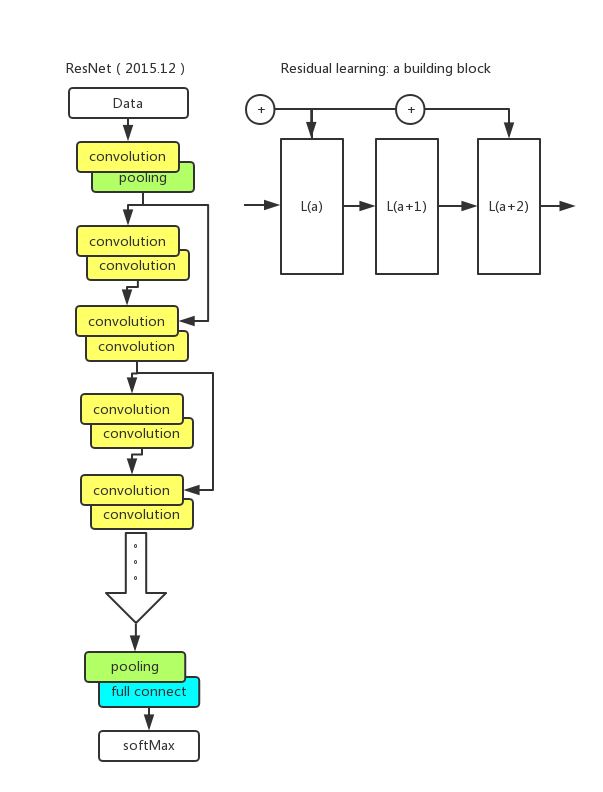
\includegraphics[width=0.5\linewidth]{picture//ResNet.png}
		% \caption{Knowledge Graph of Machine Learning}
		% \label{Fig:1}
	\end{center}
	% \vspace{-0.1em}
\end{figure}

}
	\frame{
\frametitle{ResNet}%此页的标题

\begin{figure}
	\begin{center}
		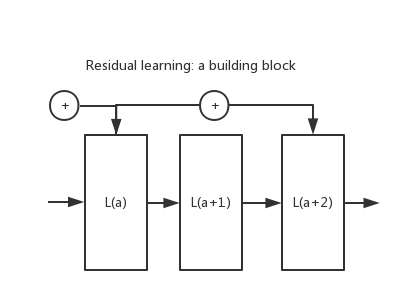
\includegraphics[width=0.3\linewidth]{picture//ResNet2.png}
		\caption{ a building block}
		% \label{ Fig:}

	\end{center}
	\vspace{-0.1em}

\end{figure}

\begin{eqnarray}
	L\left( a+1\right) &=&f\left( W\cdot L\left( a\right) +b\right)\\
	L\left( a+2\right) &=&f\left( W\cdot L\left( a+1\right) +b+L\left( a\right) \right)\\
	W&:=&W-\alpha .\dfrac {\partial J}{\partial w}\\
	\dfrac {\partial J}{\partial w}&=&\dfrac {\partial J}{\partial W_{1}}.\dfrac {\partial W_{1}}{\partial W_{2}}.\dfrac {\partial W_{2}}{\partial W_{3}}.\ldots \dfrac {\partial W_{n-1}}{\partial W_{n}}
\end{eqnarray}



}
	\frame{
\frametitle{ResNet}%此页的标题

\begin{figure}
	\begin{center}
		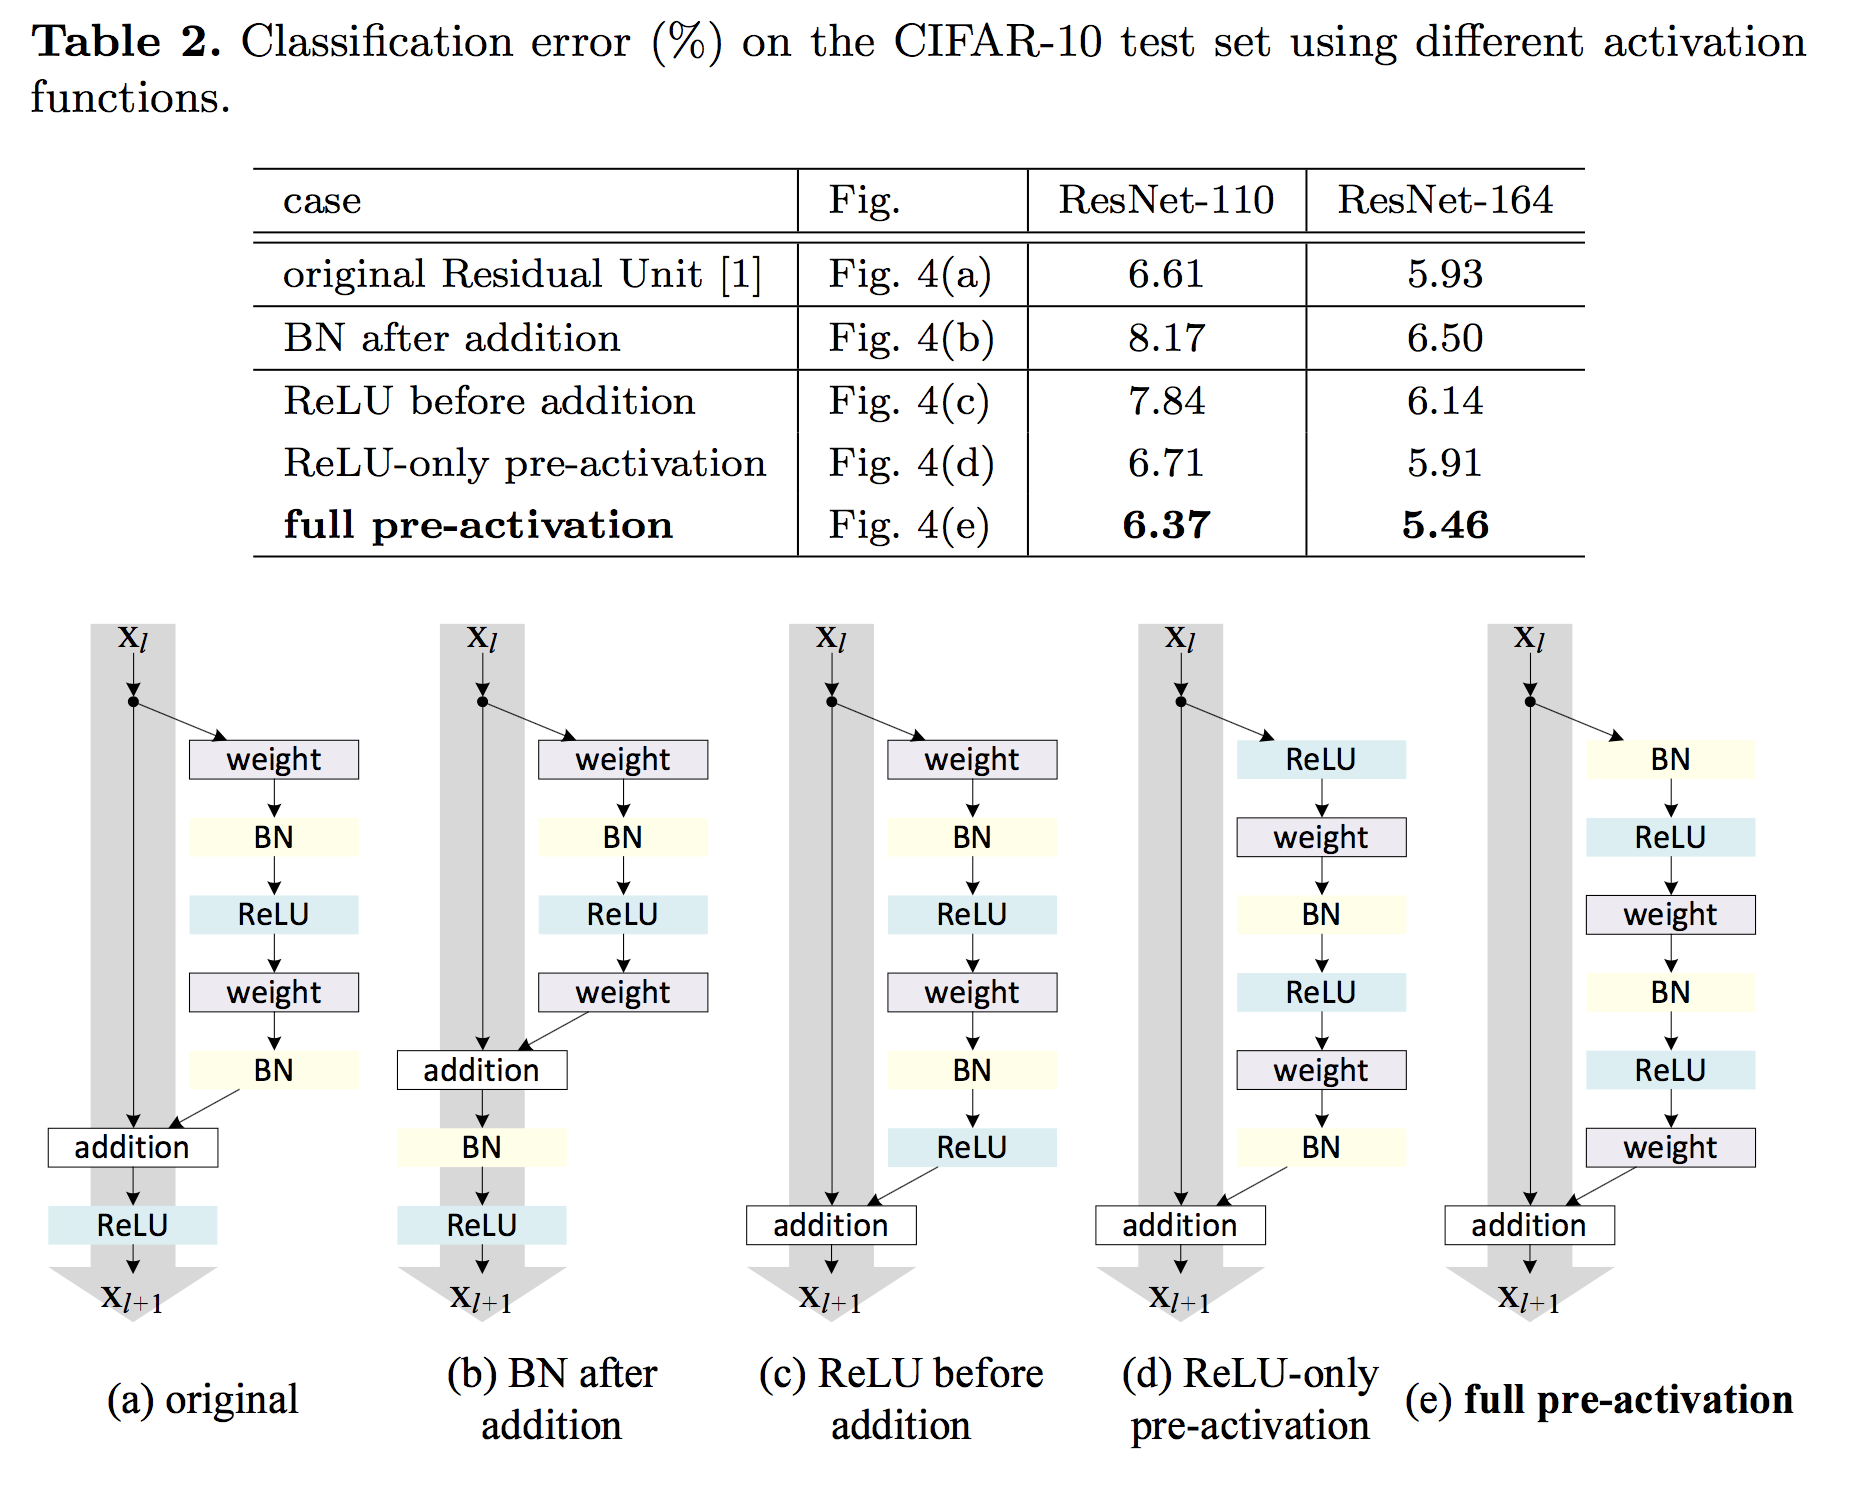
\includegraphics[width=0.7\linewidth]{picture//ResNet3.png}
		%\caption{ a building block}
		% \label{ Fig:}

	\end{center}
	\vspace{-0.1em}

\end{figure}

}
	\frame{
\frametitle{Inception-V3}%此页的标题

\begin{figure}
	\begin{center}
		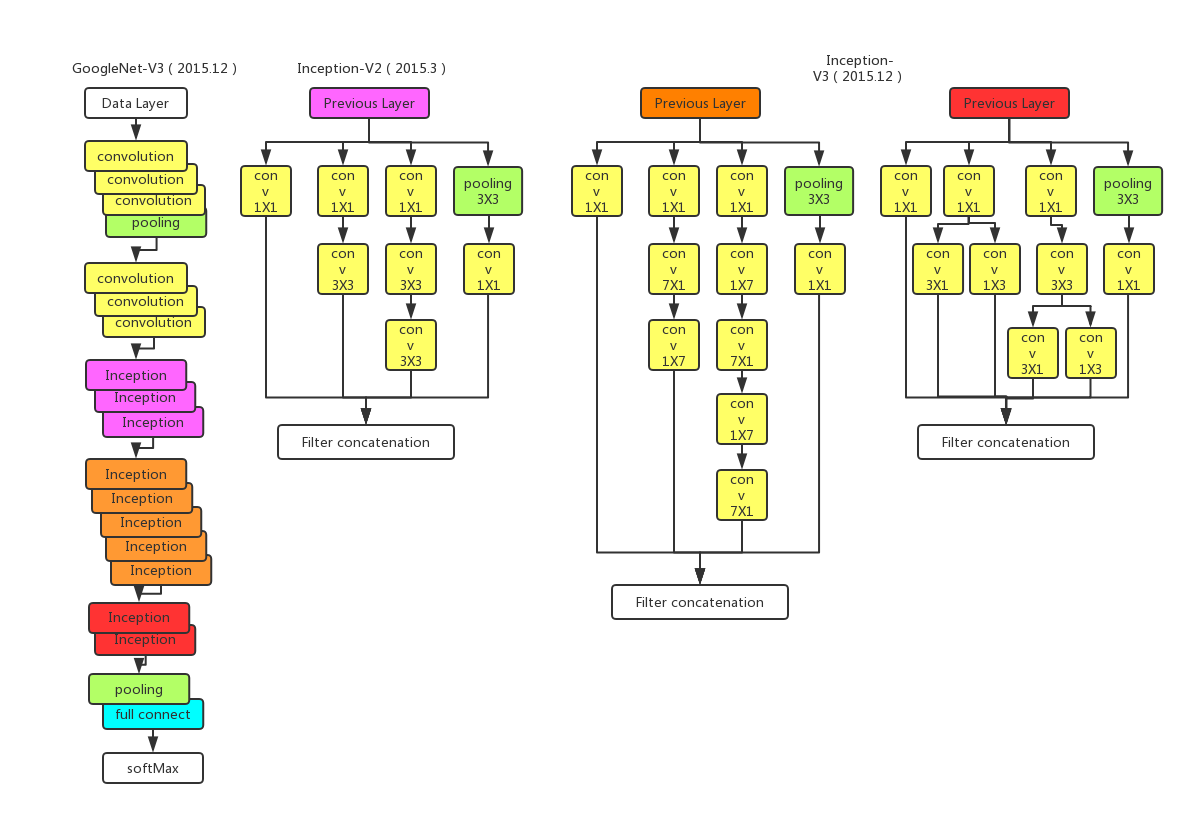
\includegraphics[width=1\linewidth]{picture//InceptionV3.png}
		% \caption{Knowledge Graph of Machine Learning}
		% \label{Fig:1}
	\end{center}
	% \vspace{-0.1em}
\end{figure}

}
	\frame{
\frametitle{Inception-V4}%此页的标题

\begin{figure}
	\begin{center}
		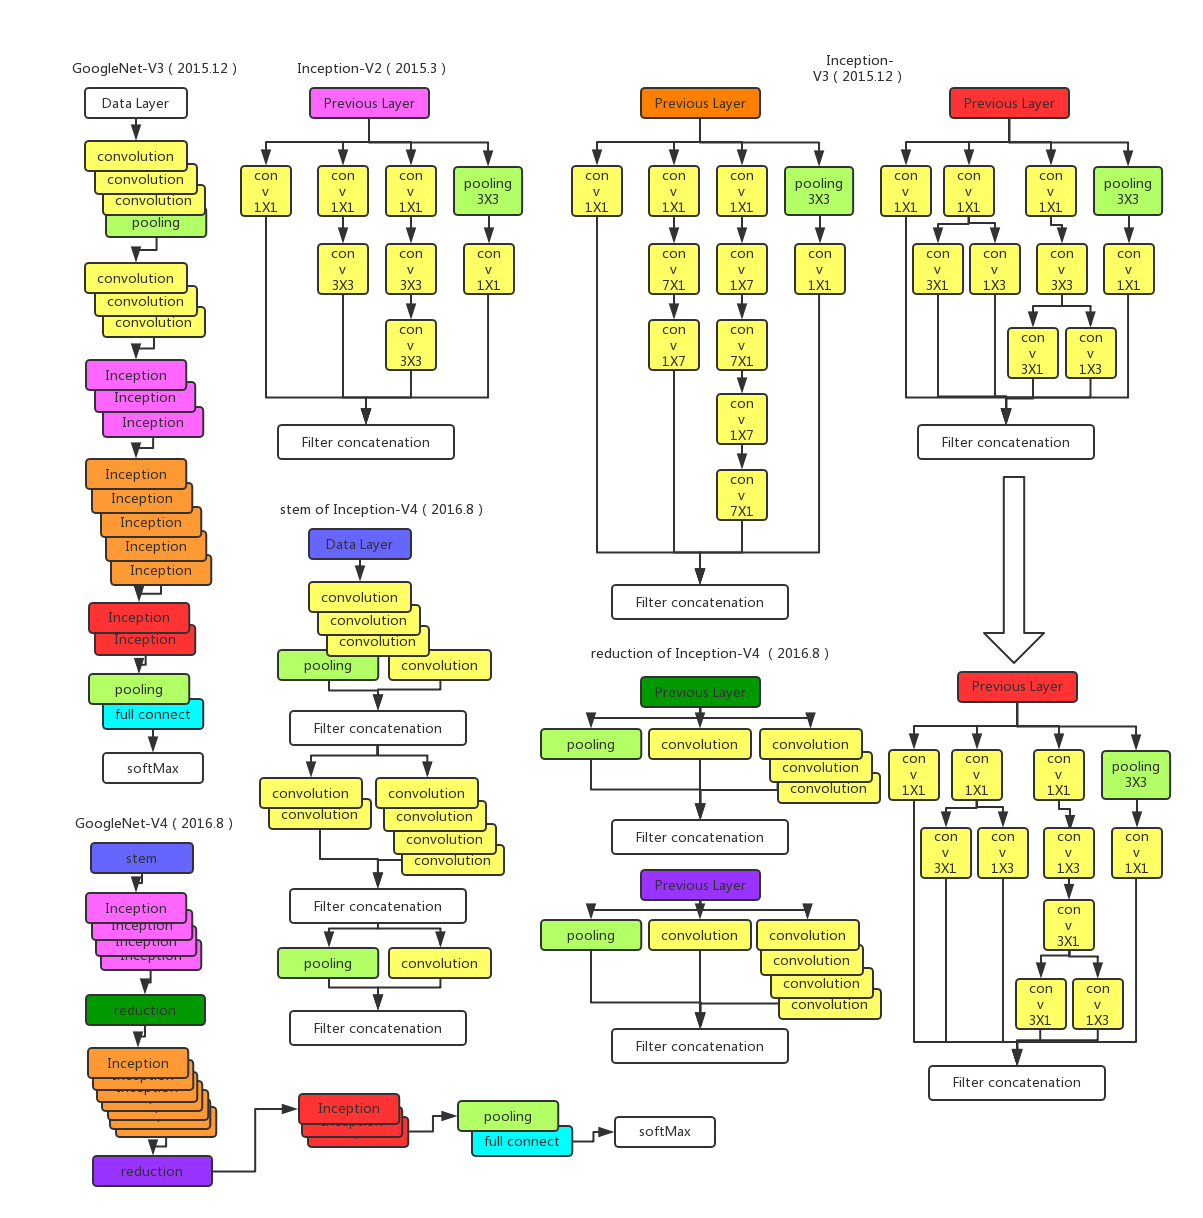
\includegraphics[width=0.6\linewidth]{picture//InceptionV4.png}
		% \caption{Knowledge Graph of Machine Learning}
		% \label{Fig:1}
	\end{center}
	% \vspace{-0.1em}
\end{figure}

}
	\frame{
\frametitle{Inception-ResNet-V2}%此页的标题

\begin{figure}
	\begin{center}
		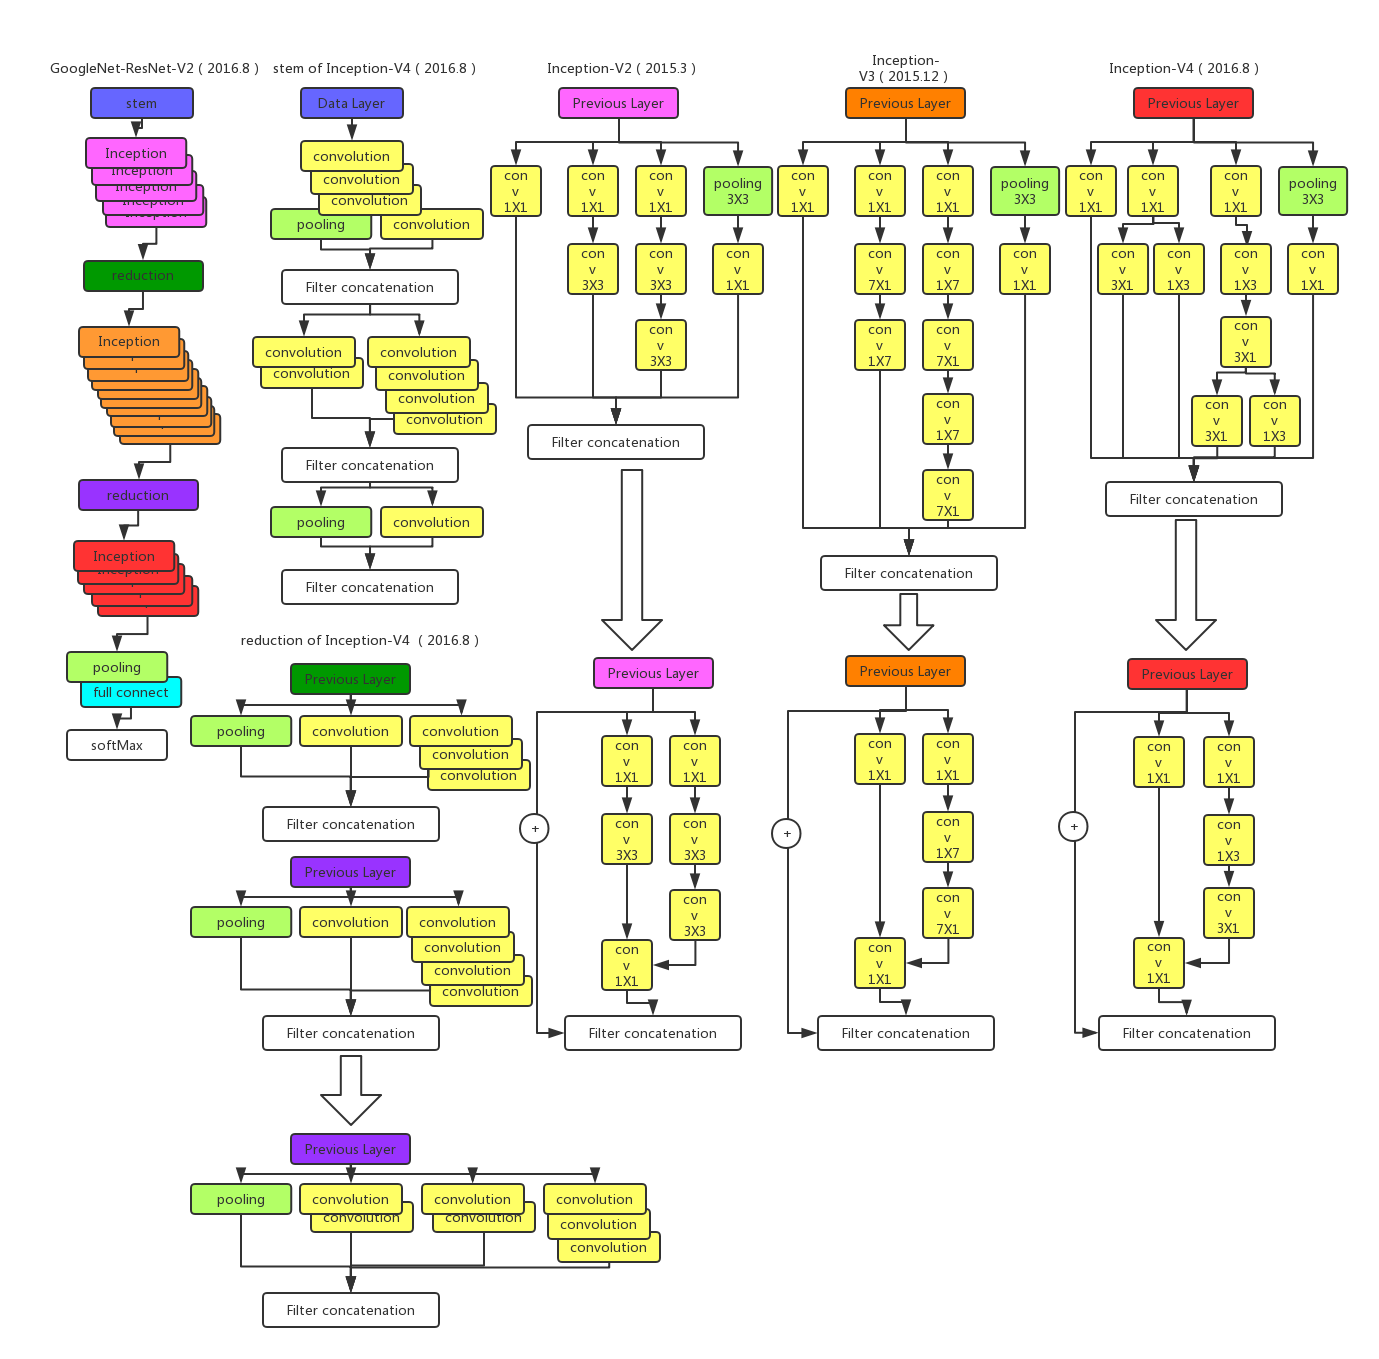
\includegraphics[width=0.7\linewidth]{picture//InceptionResNetV2.png}
		%\caption{ a building block}
		% \label{ Fig:}

	\end{center}
	\vspace{-0.1em}

\end{figure}

}
	\frame{
\frametitle{Inception-ResNet-V2}%此页的标题

\begin{figure}
	\begin{center}
		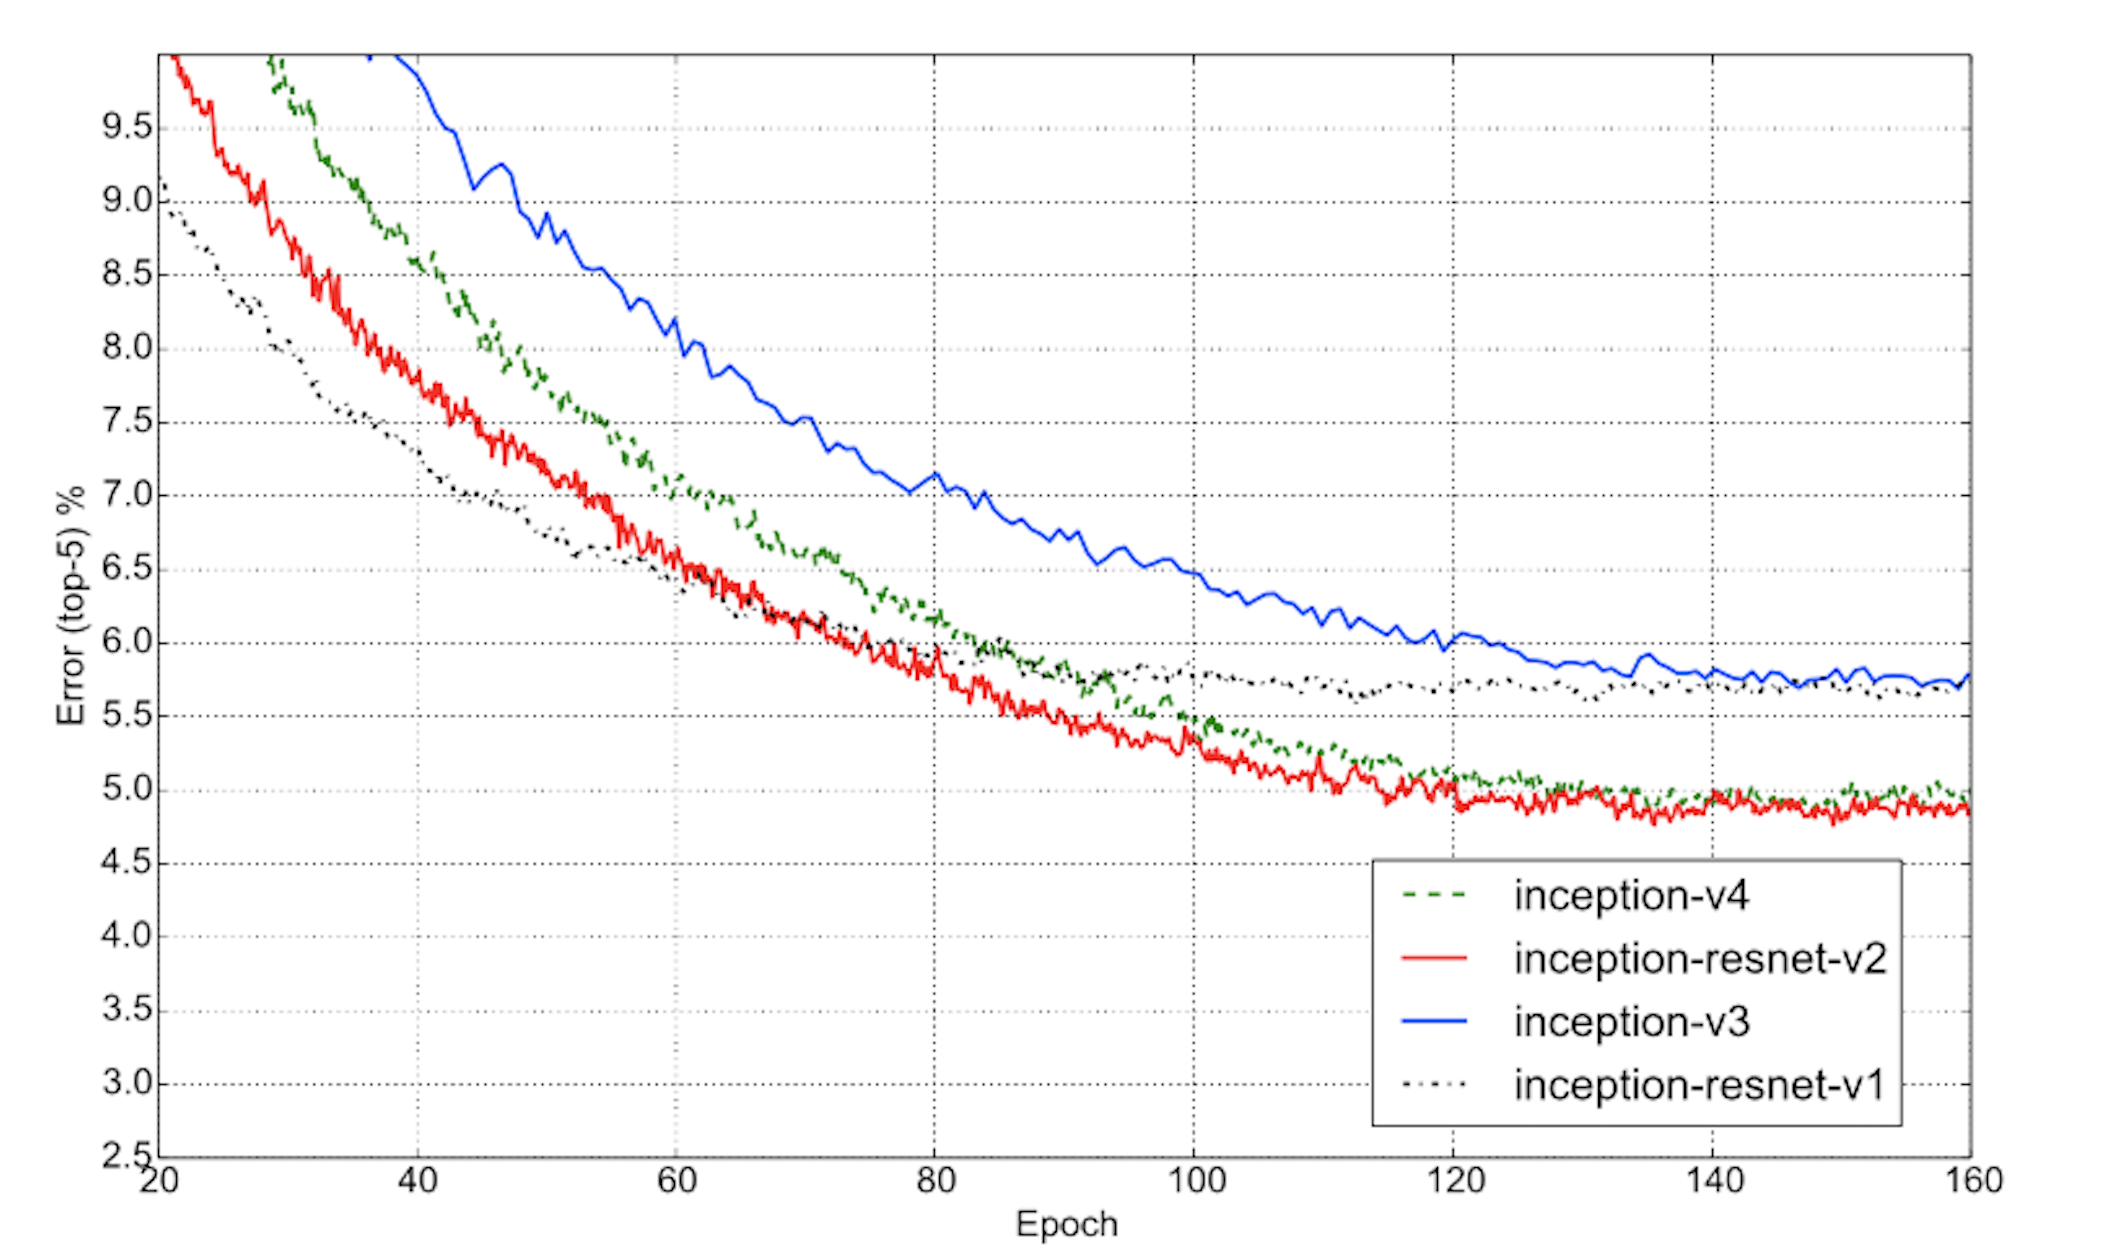
\includegraphics[width=0.8\linewidth]{picture//result.png}
		\caption{Large Scale Visual Recognition Challenge 2012 (ILSVRC2012)}
		\label{Fig:1}
	\end{center}
	% \vspace{-0.1em}
\end{figure}

}
	\frame{
\frametitle{FractalNet}%此页的标题

\begin{figure}
	\begin{center}
		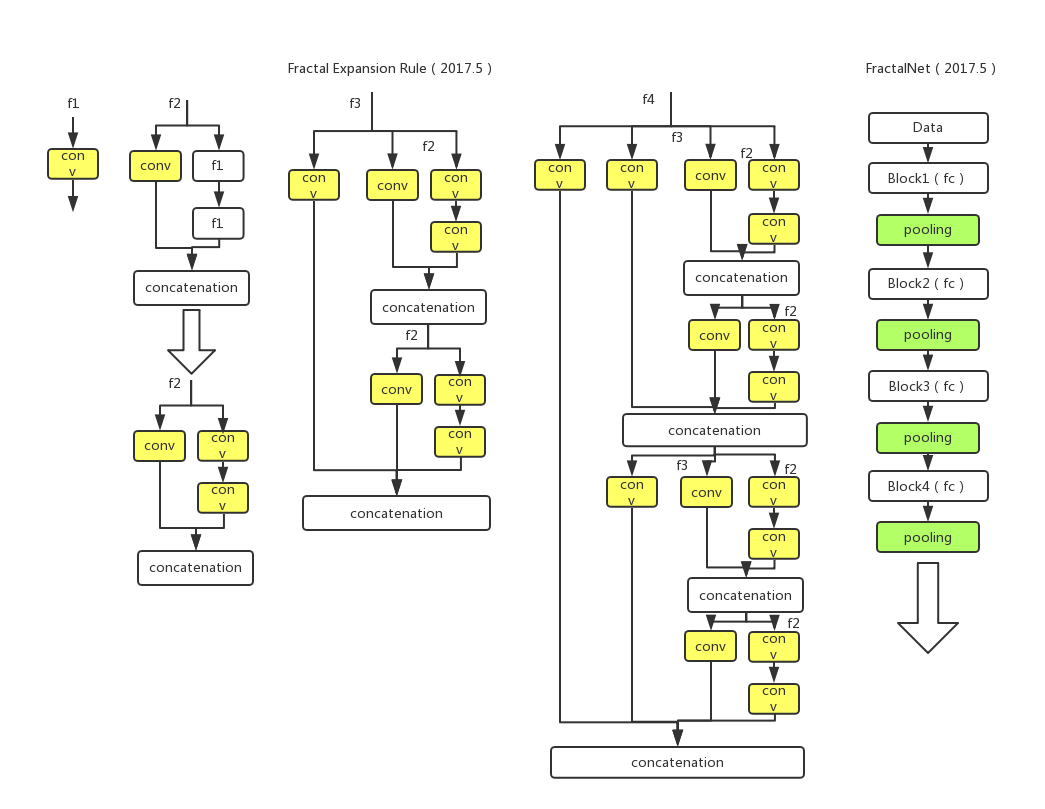
\includegraphics[width=0.9\linewidth]{picture//FractalNet.png}
		%\caption{Large Scale Visual Recognition Challenge 2012 (ILSVRC2012)}
		% \label{Fig:1}
	\end{center}
	% \vspace{-0.1em}
\end{figure}

}
	\frame{
\frametitle{FractalNet}%此页的标题

\begin{figure}
	\begin{center}
		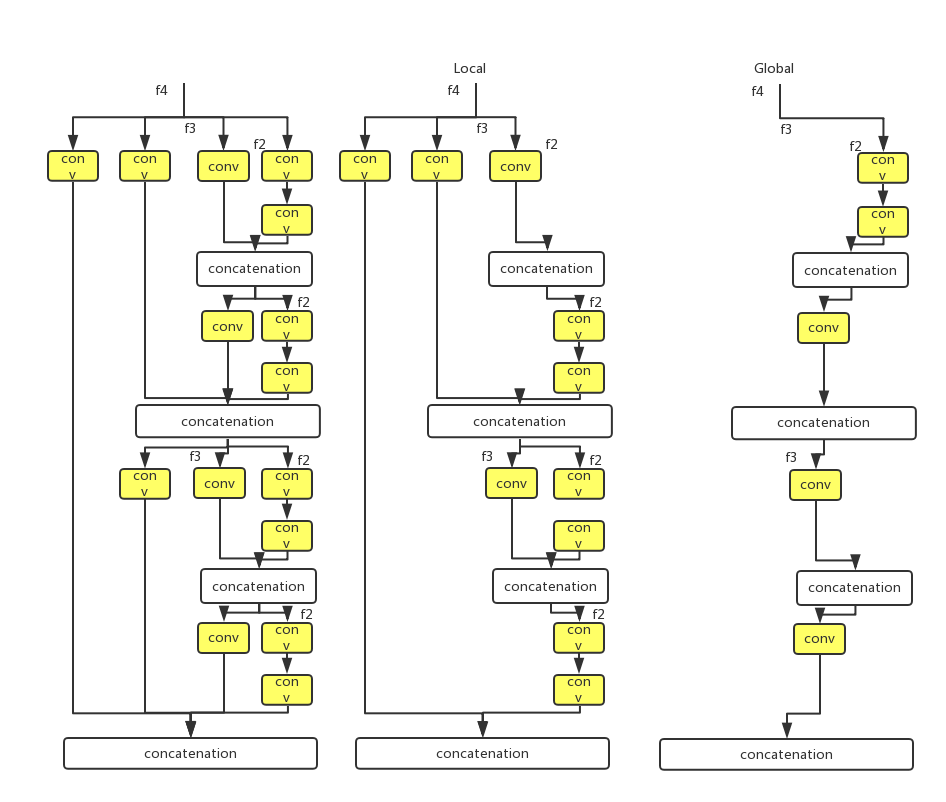
\includegraphics[width=0.7\linewidth]{picture//DropPath.png}
		\caption{Drop-Path}
		 \label{Fig:2}
	\end{center}
	% \vspace{-0.1em}
\end{figure}

}
	\frame{
\frametitle{DenseNet 2017.8}%此页的标题

\begin{figure}
	\begin{center}
		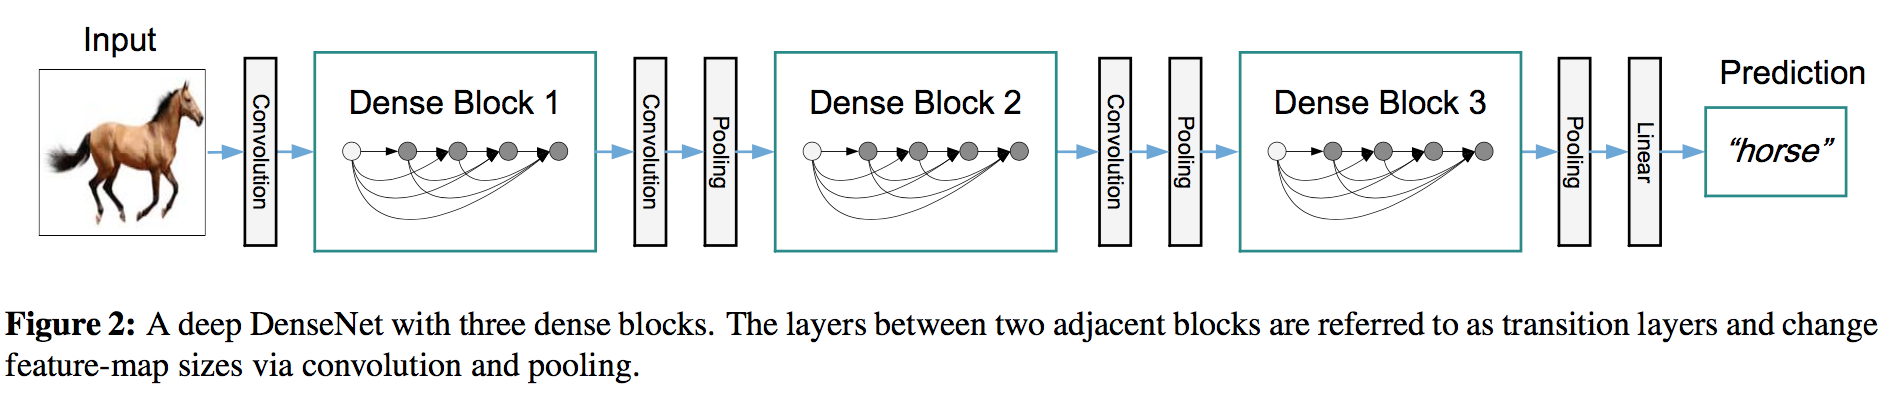
\includegraphics[width=1\linewidth]{picture//DenseNet.png}
		% \caption{Drop-Path}
		 % \label{Fig:2}
	\end{center}
	% \vspace{-0.1em}
\end{figure}

\begin{itemize}

\item \justifying Accuracy

\item The number of parameters

\item Overfitting or the optimization difficulties

\end{itemize}

}

	% \section{Layer-CNN}%第二标题
	% \subsection{FakeTitle1} % subtitles are not used in this layout but still required for the header outline bullets
	% \frame{
\frametitle{Latex}%此页的标题

\begin{figure}
	\begin{center}
		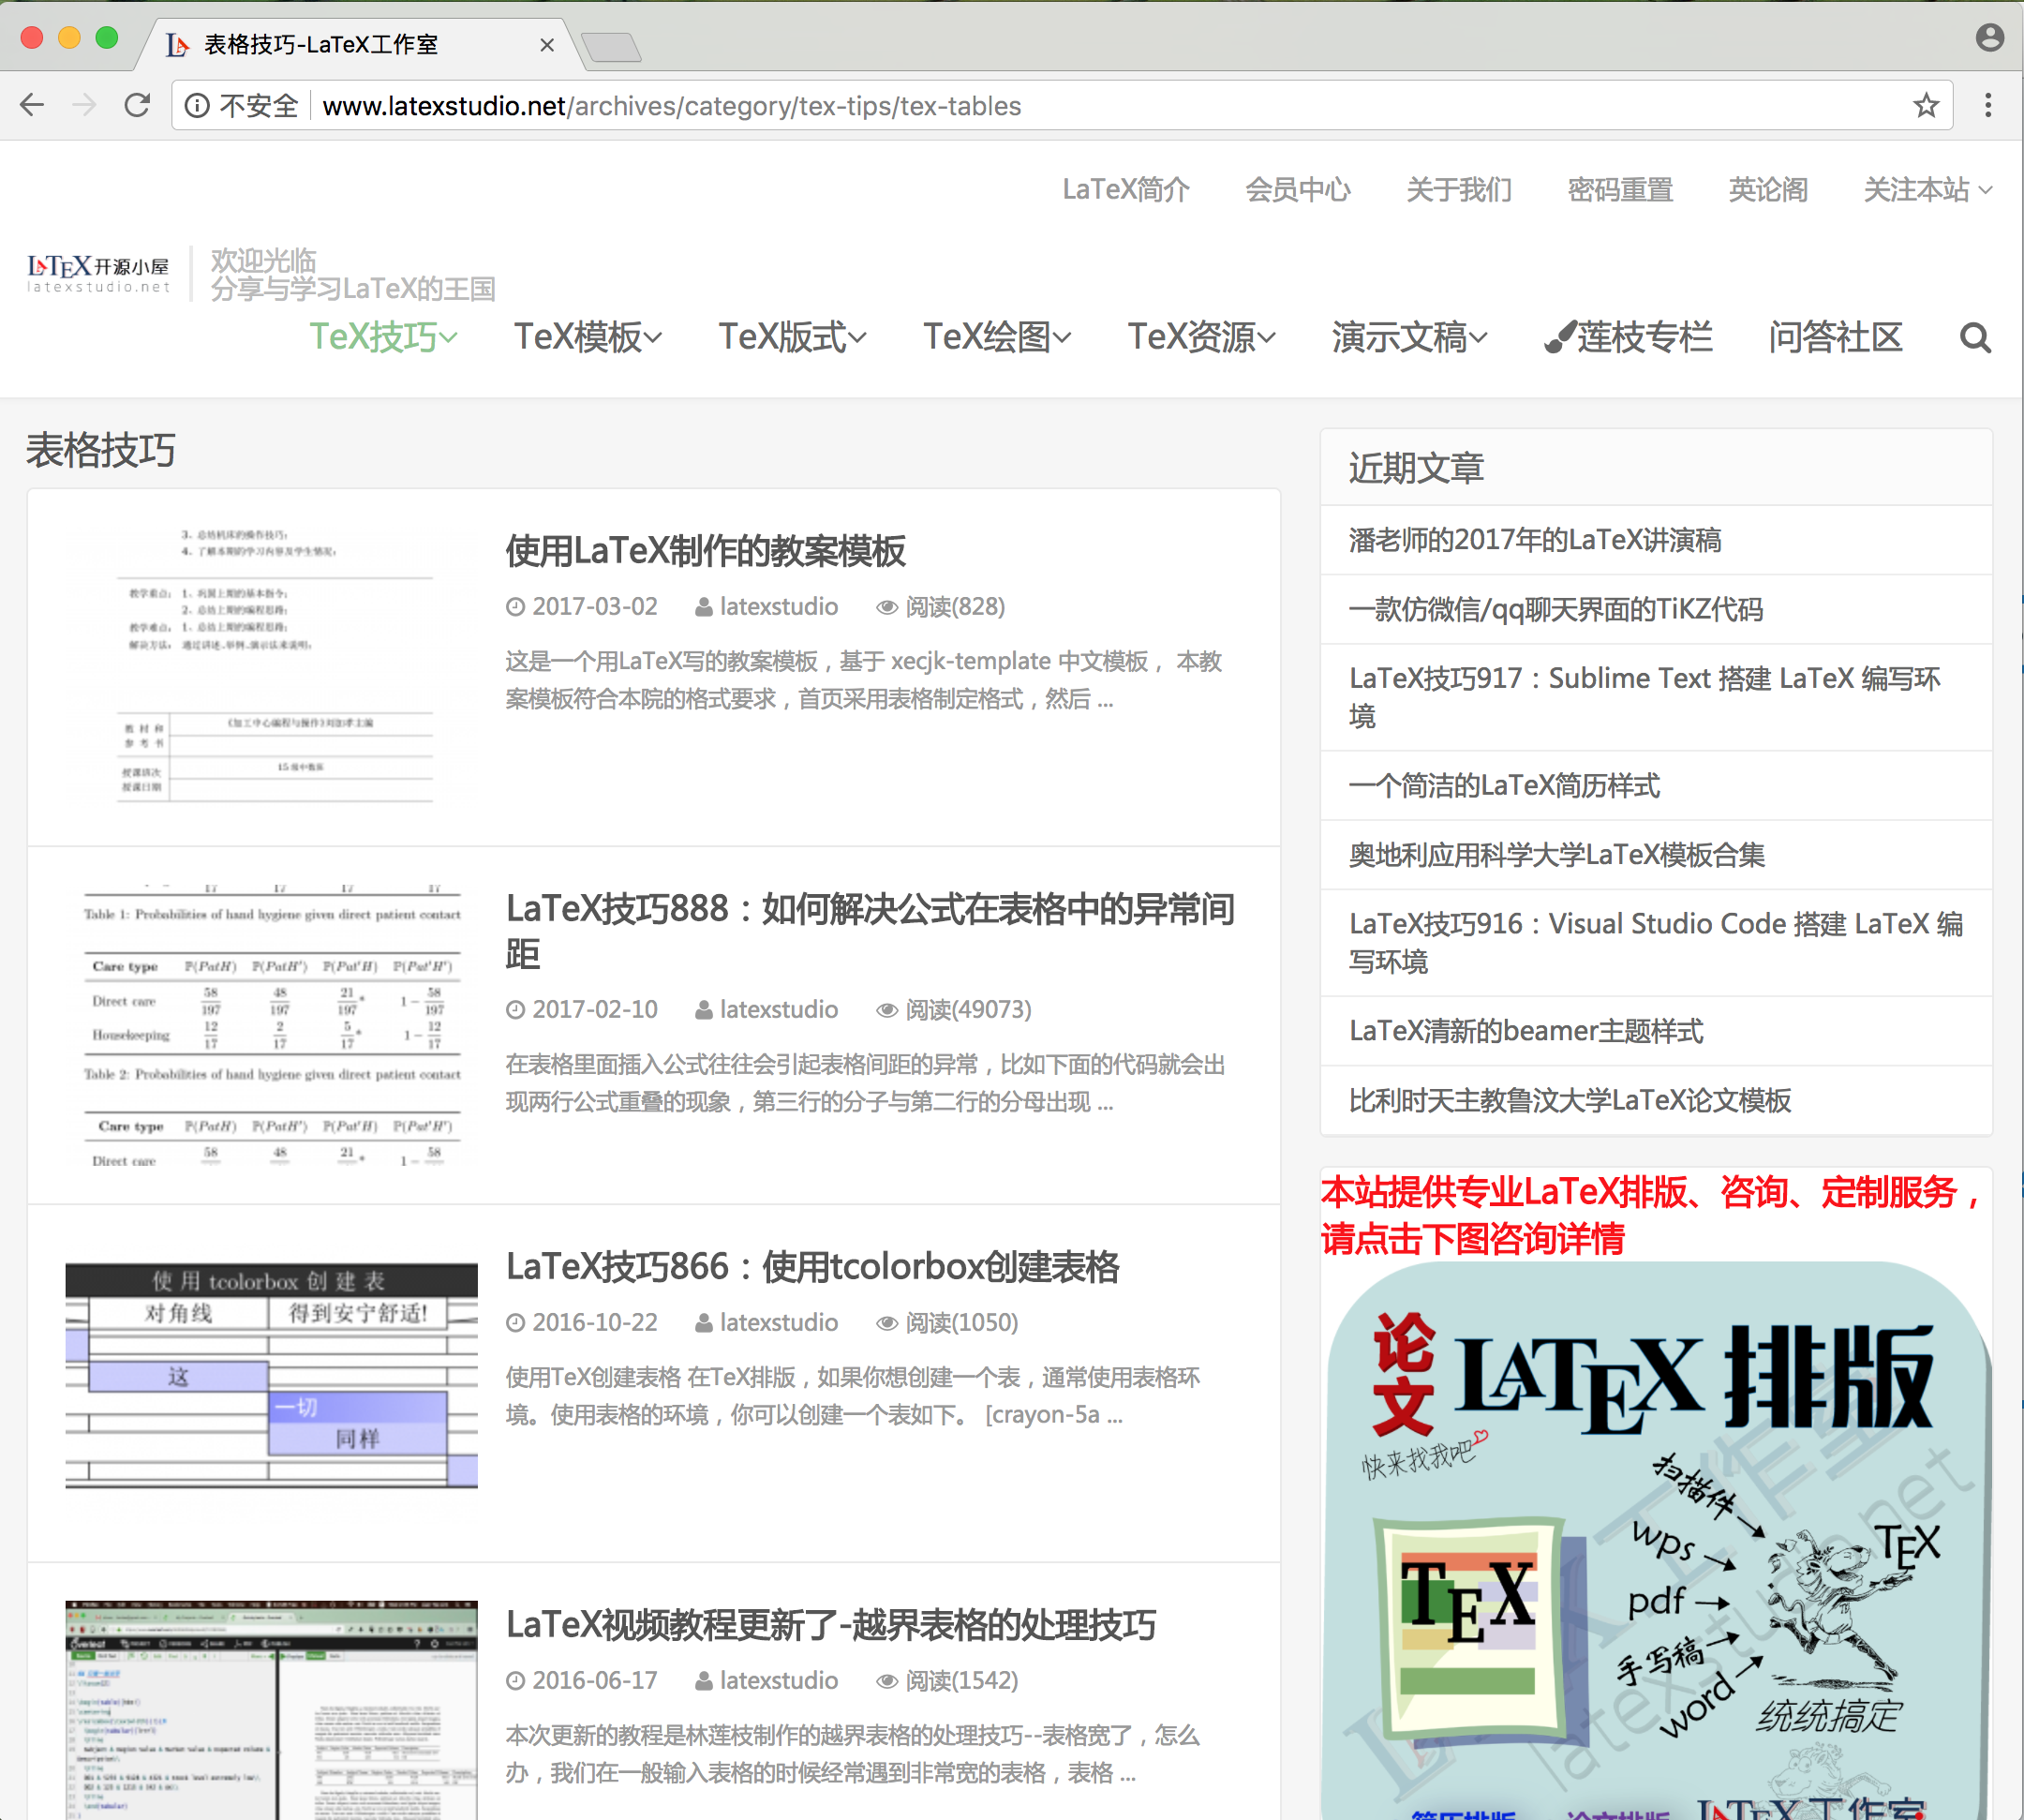
\includegraphics[width=0.6\linewidth]{picture//pic3.png}
		\caption{http://www.latexstudio.net/}
		\label{Fig:1}
	\end{center}
	% \vspace{-0.1em}
\end{figure}

}


	% \frame{
\frametitle{Latex}%此页的标题

\begin{figure}
	\begin{center}
		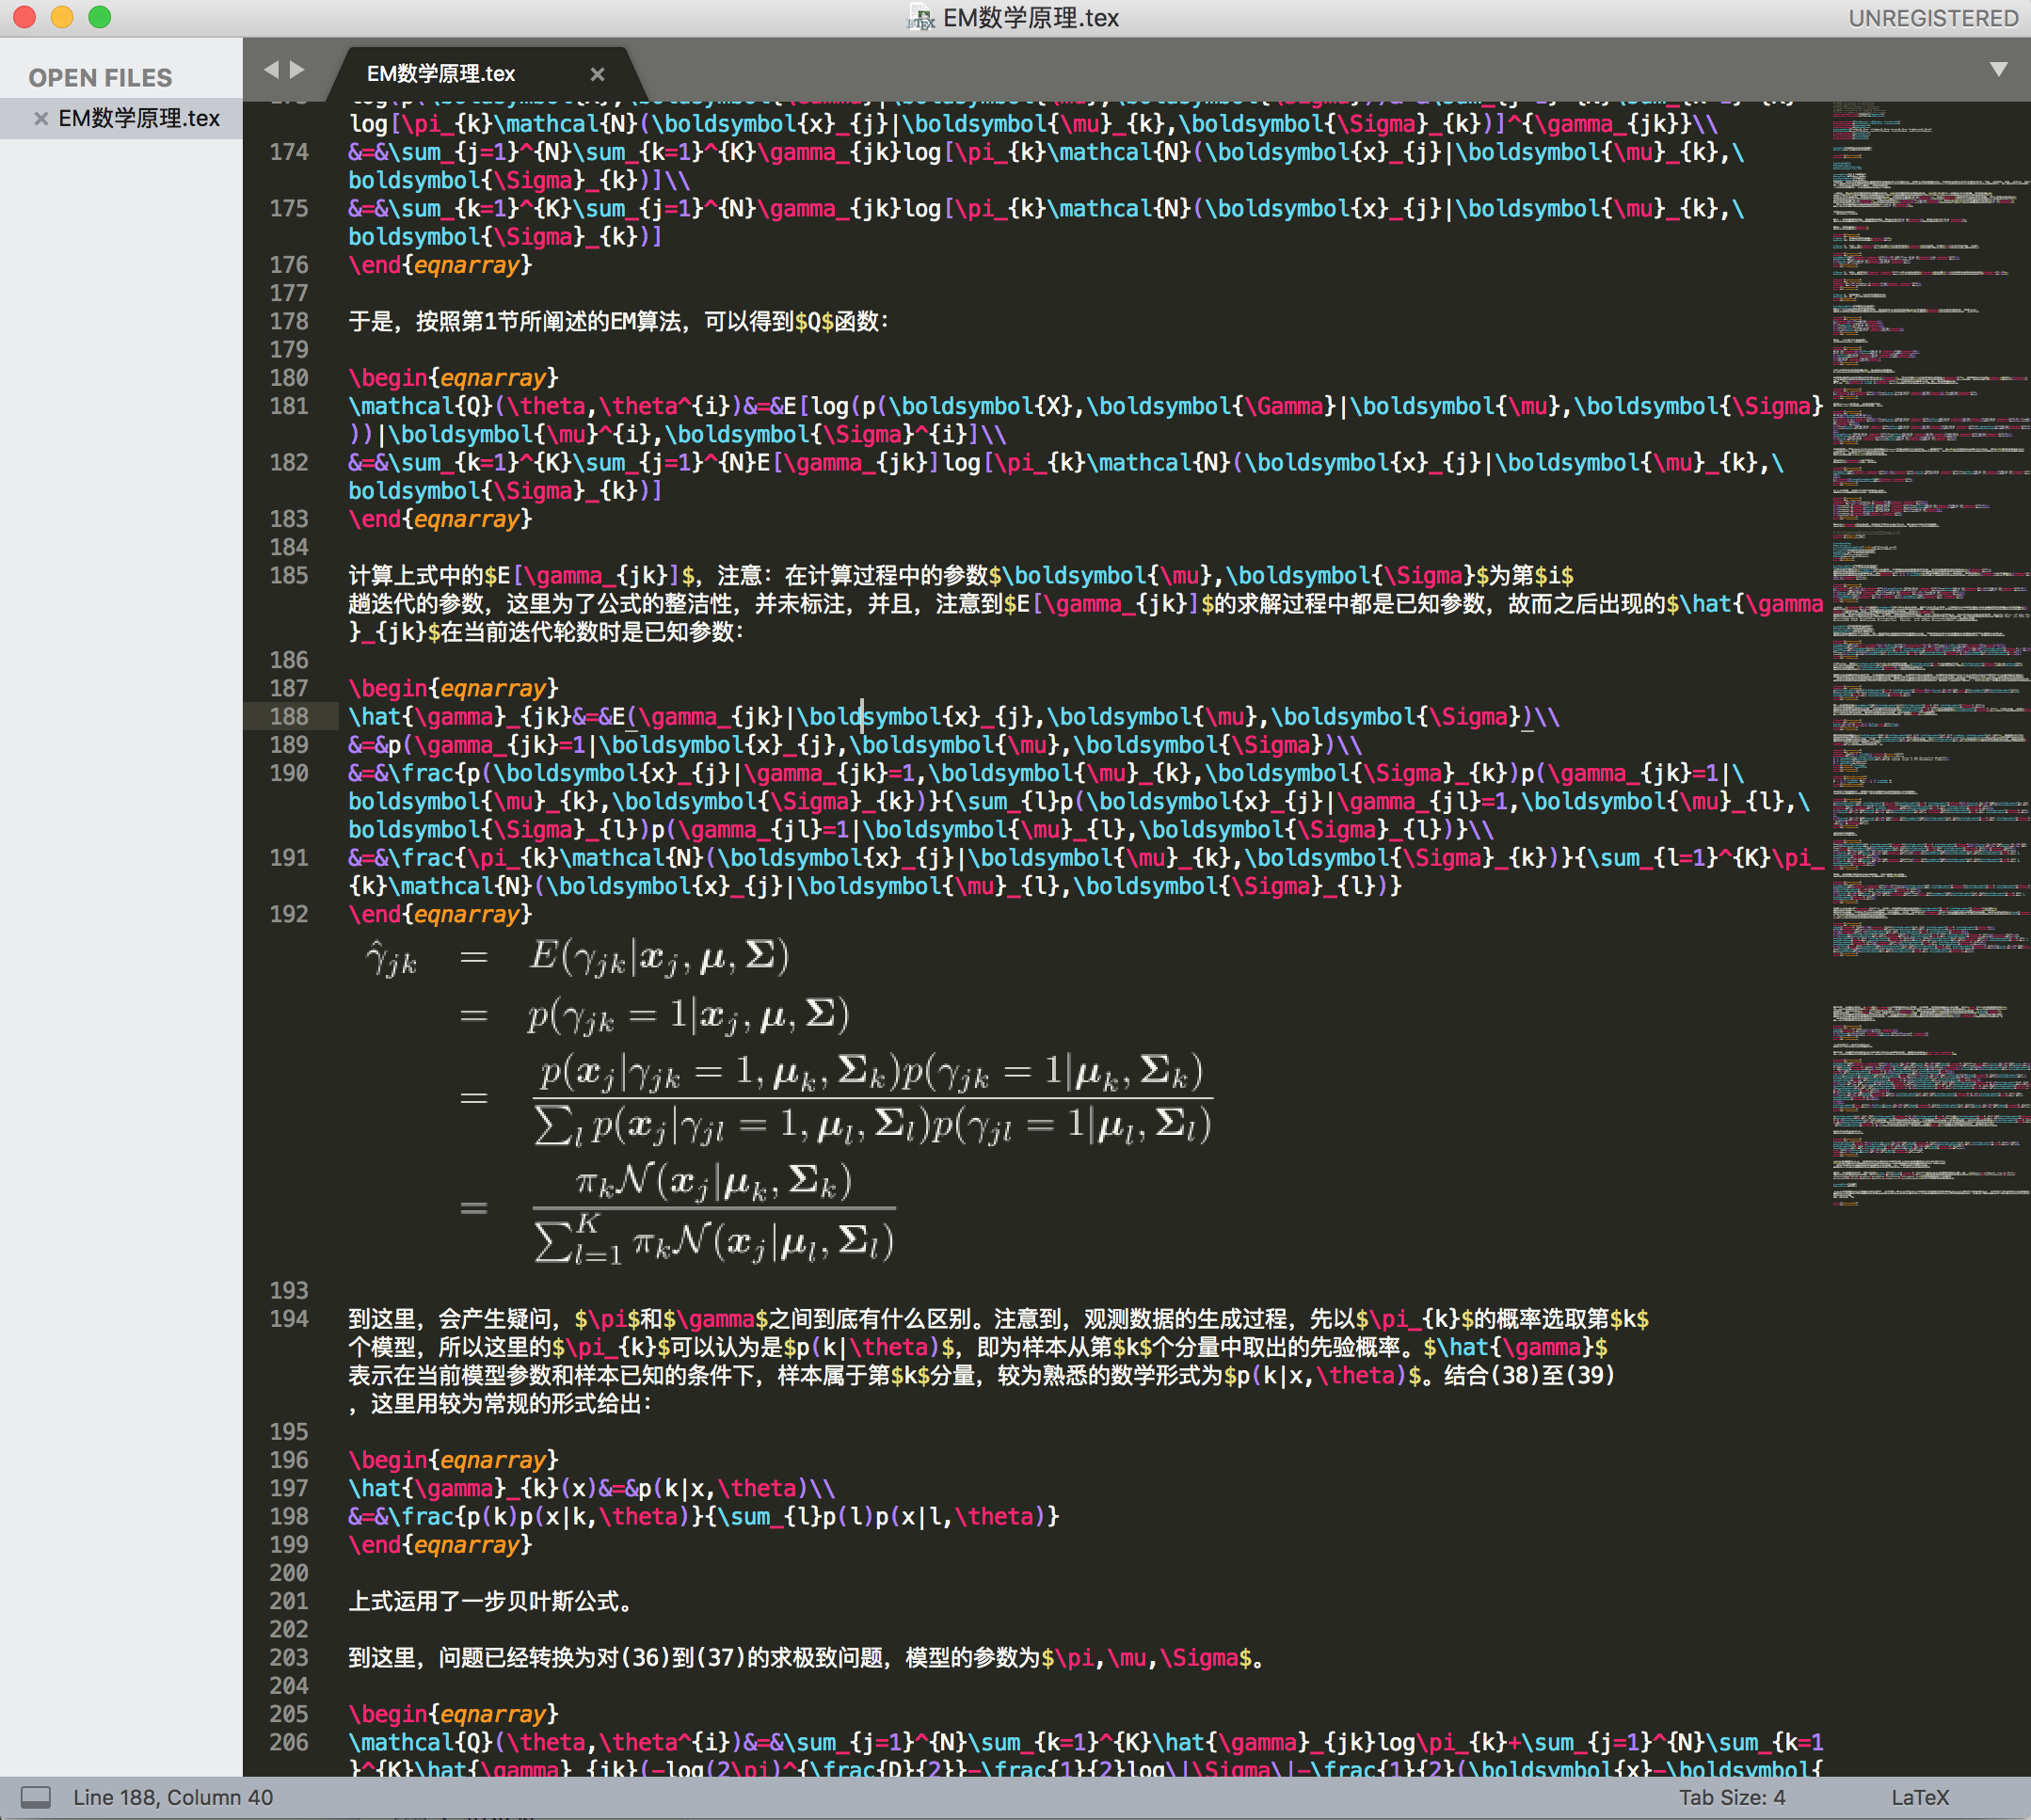
\includegraphics[width=0.6\linewidth]{picture//pic4.png}
		\caption{Sublime Text3}
		\label{Fig:1}
	\end{center}
	% \vspace{-0.1em}
\end{figure}

}
	%\section{TensorFlow}
	%\subsection{FakeTitle1} % subtitles are not used in this layout but still required for the header outline bullets
	%

	\section{Latex}%第三标题
	\subsection{FakeTitle1} % subtitles are not used in this layout but still required for the header outline bullets
	\frame{
\frametitle{Latex}%此页的标题

\begin{figure}
	\begin{center}
		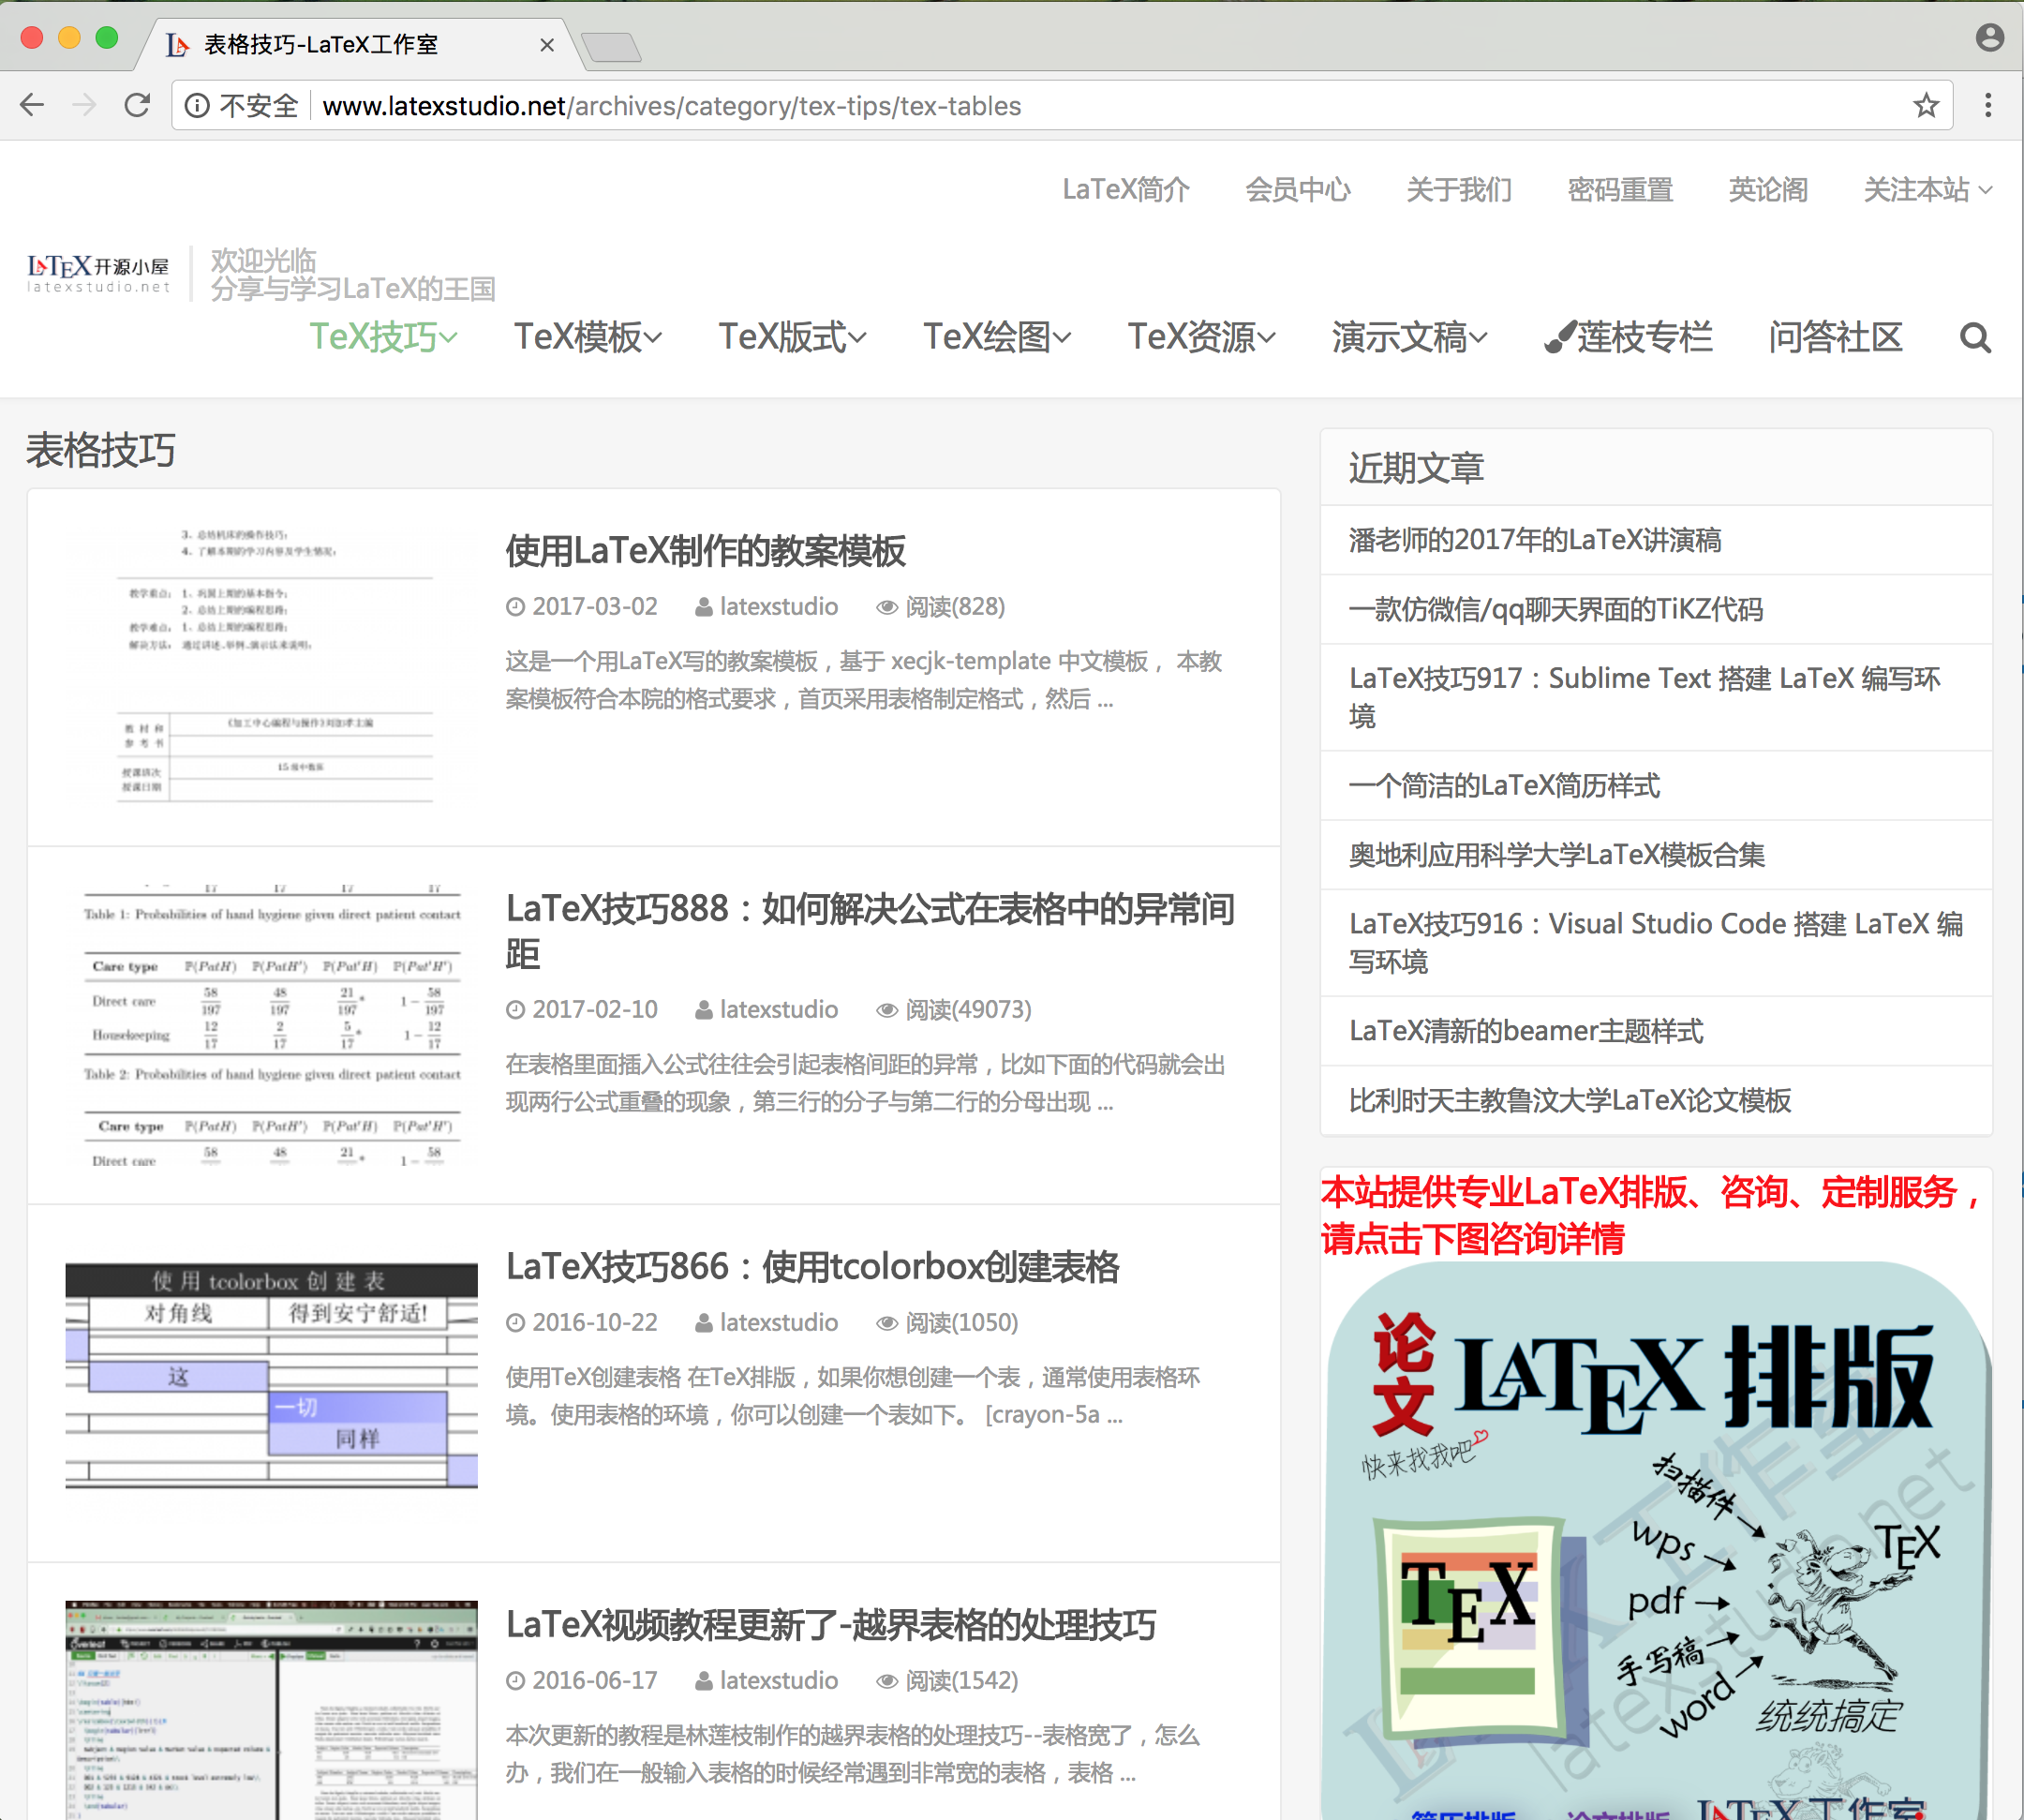
\includegraphics[width=0.6\linewidth]{picture//pic3.png}
		\caption{http://www.latexstudio.net/}
		\label{Fig:1}
	\end{center}
	% \vspace{-0.1em}
\end{figure}

}


	\frame{
\frametitle{Latex}%此页的标题

\begin{figure}
	\begin{center}
		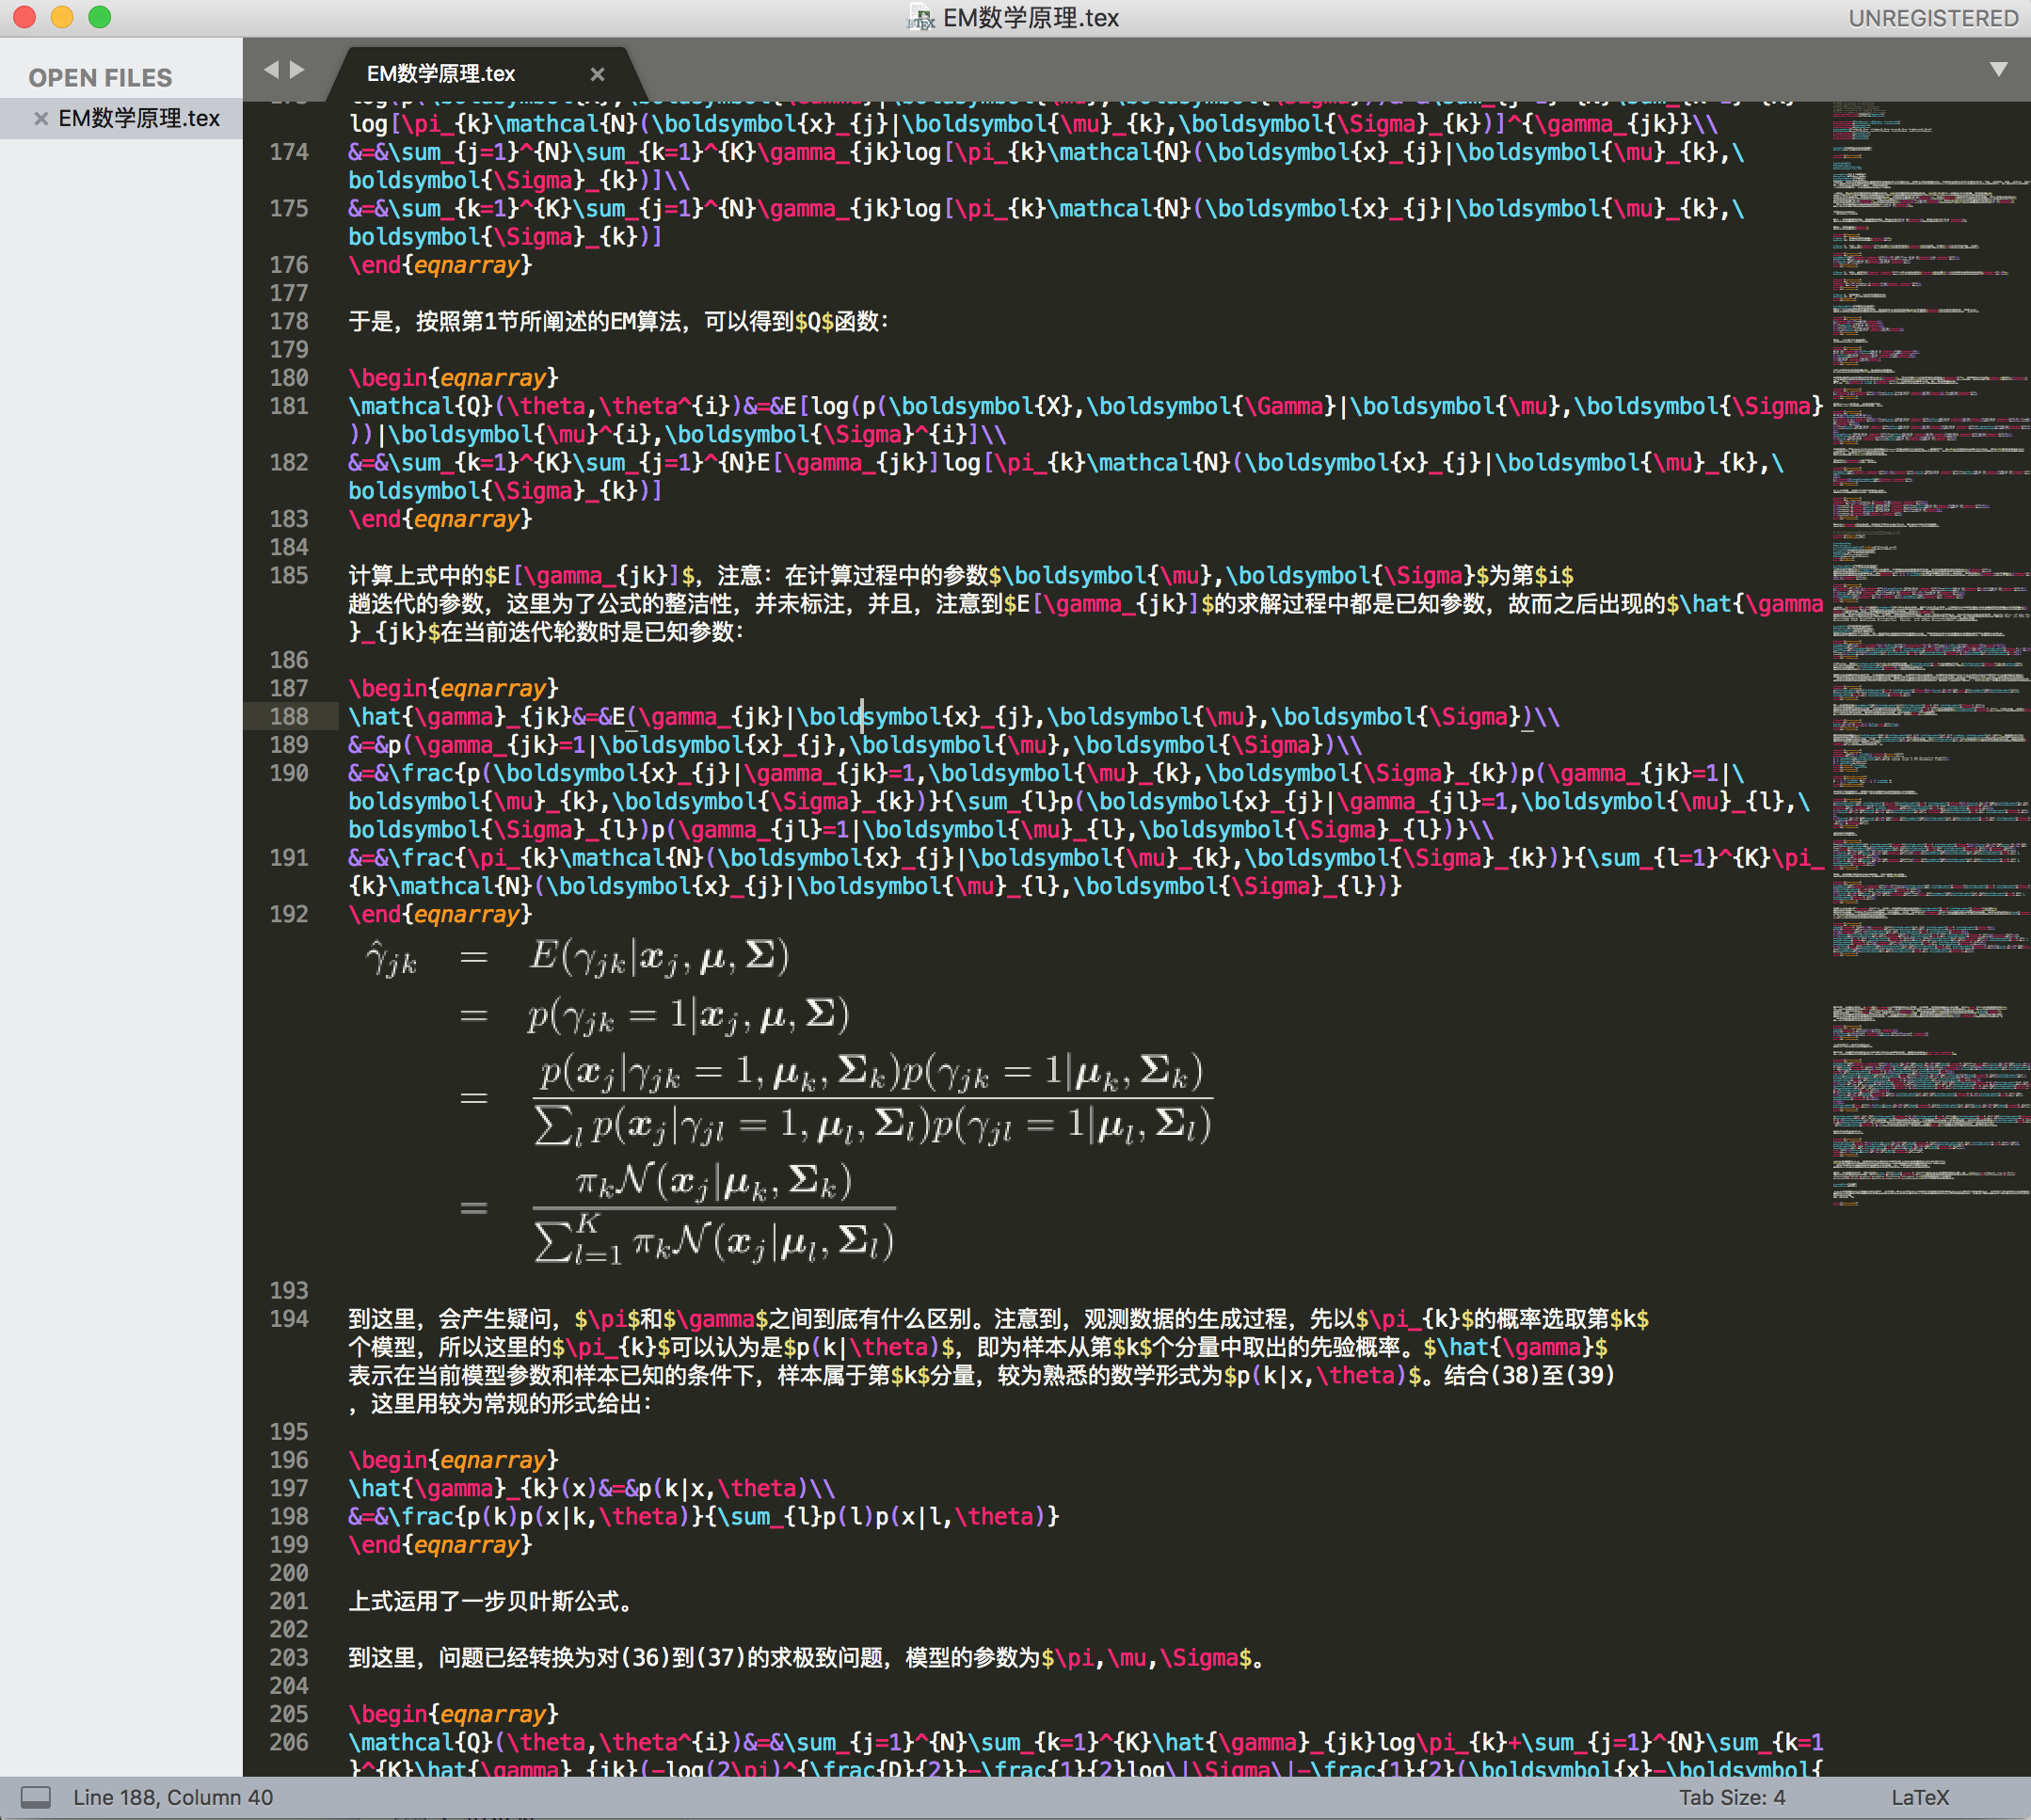
\includegraphics[width=0.6\linewidth]{picture//pic4.png}
		\caption{Sublime Text3}
		\label{Fig:1}
	\end{center}
	% \vspace{-0.1em}
\end{figure}

}

\end{document}
